\section{Nonlinear probes}
\label{app:nonlinear}

Weak linear recovery does not imply that a representation lacks the target
information. LeWM's original study also uses nonlinear probes to assess
physical quantities \citep{maes2026leworldmodel}. We therefore fit a small MLP
to the same frozen states and endpoint targets used in the main paper.
The network has two 256-unit ReLU hidden layers and jointly predicts the
16 coordinates of the four positional and four cue-indexed endpoints.

We use 512 fit episodes, 128 validation episodes, and 256 episodes held out from probe
fitting. Feature and coordinate normalization use only the fit episodes.
For each of three probe initialization seeds, validation error selects the
learning rate ($10^{-3}$ or $3\times10^{-4}$), AdamW weight decay (0 or .01),
and stopping epoch. Training uses full batches of 512, at most 1,000 epochs,
and a patience of 100 epochs. Selection minimizes the mean squared error of
standardized coordinates across all targets. A ridge comparator uses the
same fit/validation split and selects its penalty from
$\{.01,.1,1,10,100,1000\}$; all six state/variant combinations select 100.
Test results are evaluated after these choices are fixed.

\begin{table}[!htbp]
\centering
\caption{\textbf{A small nonlinear probe leaves the location--cue gap largely intact.}
Metrics average four endpoints. MLP entries show mean $\pm$ sample SD
across three probe initializations, not world-model training runs. Both
methods fit 512 episodes; the main paper's fixed-penalty ridge uses 640.}
\label{tab:nonlinear}
\renewcommand{\arraystretch}{1.12}
\setlength{\tabcolsep}{3pt}
\begin{tabular*}{\linewidth}{@{\extracolsep{\fill}}llrrrr@{}}
\toprule
Variant & Probe & Cue MAE $\downarrow$ & Cue $R^2\uparrow$ & Location MAE $\downarrow$ & Location $R^2\uparrow$ \\
\midrule
\multicolumn{6}{l}{\emph{Current projected states}} \\
Color & Ridge & $27.48$ & $.262$ & $4.05$ & $.923$ \\
Color & MLP & $27.50\pm0.03$ & $.273\pm.005$ & $5.09\pm0.16$ & $.885\pm.006$ \\
Shape & Ridge & $27.91$ & $.250$ & $4.85$ & $.894$ \\
Shape & MLP & $27.74\pm0.07$ & $.261\pm.006$ & $5.76\pm0.13$ & $.857\pm.003$ \\
Palette & Ridge & $27.43$ & $.271$ & $4.24$ & $.913$ \\
Palette & MLP & $27.78\pm0.12$ & $.259\pm.003$ & $5.32\pm0.14$ & $.874\pm.005$ \\
\midrule
\multicolumn{6}{l}{\emph{One-step predicted states}} \\
Color & Ridge & $27.42$ & $.267$ & $3.92$ & $.926$ \\
Color & MLP & $27.53\pm0.06$ & $.273\pm.004$ & $5.03\pm0.14$ & $.887\pm.007$ \\
Shape & Ridge & $27.83$ & $.258$ & $4.72$ & $.900$ \\
Shape & MLP & $27.73\pm0.10$ & $.262\pm.005$ & $5.61\pm0.15$ & $.864\pm.004$ \\
Palette & Ridge & $27.58$ & $.270$ & $4.04$ & $.919$ \\
Palette & MLP & $27.80\pm0.14$ & $.260\pm.001$ & $5.18\pm0.18$ & $.881\pm.006$ \\
\bottomrule
\end{tabular*}
\end{table}

The MLP reaches cue $R^2=.259$--$.273$ for current states, while location
$R^2$ remains much higher at $.857$--$.885$ (Table~\ref{tab:nonlinear}). Its cue
scores are close to the validation-selected ridge baseline, and its location
scores are lower. The same pattern holds for predicted states. Within this
probe family and label budget, adding nonlinearity does not close the gap.
Larger probes or more labeled episodes could give different results; these
tests do not establish information loss.

\section{Controlled portal swaps and predicted crossings}
\label{app:portal-swap}

We exchange the two central-room portal endpoints to separate encoder
sensitivity from prediction of their consequences. Unordered locations stay
fixed, while visible identities and the destination reached from each entrance
switch together. Destination-room endpoints remain unchanged. Both worlds
are physically coherent: the intervention changes visible cues along with routing.

We use 16 planning geometries, eight per rank, with identical geometry and
actions across renderings. Figure~\ref{fig:swap-states} illustrates a separate
training geometry, excluded from all aggregates. Controls translate either
the agent or both central-room endpoints by eight pixels; the latter changes
occupied geometry while preserving identities. We measure squared projected-state
distance from the original observation, with same-state distance as a zero
reference.

\begin{figure}[!htbp]
\centering
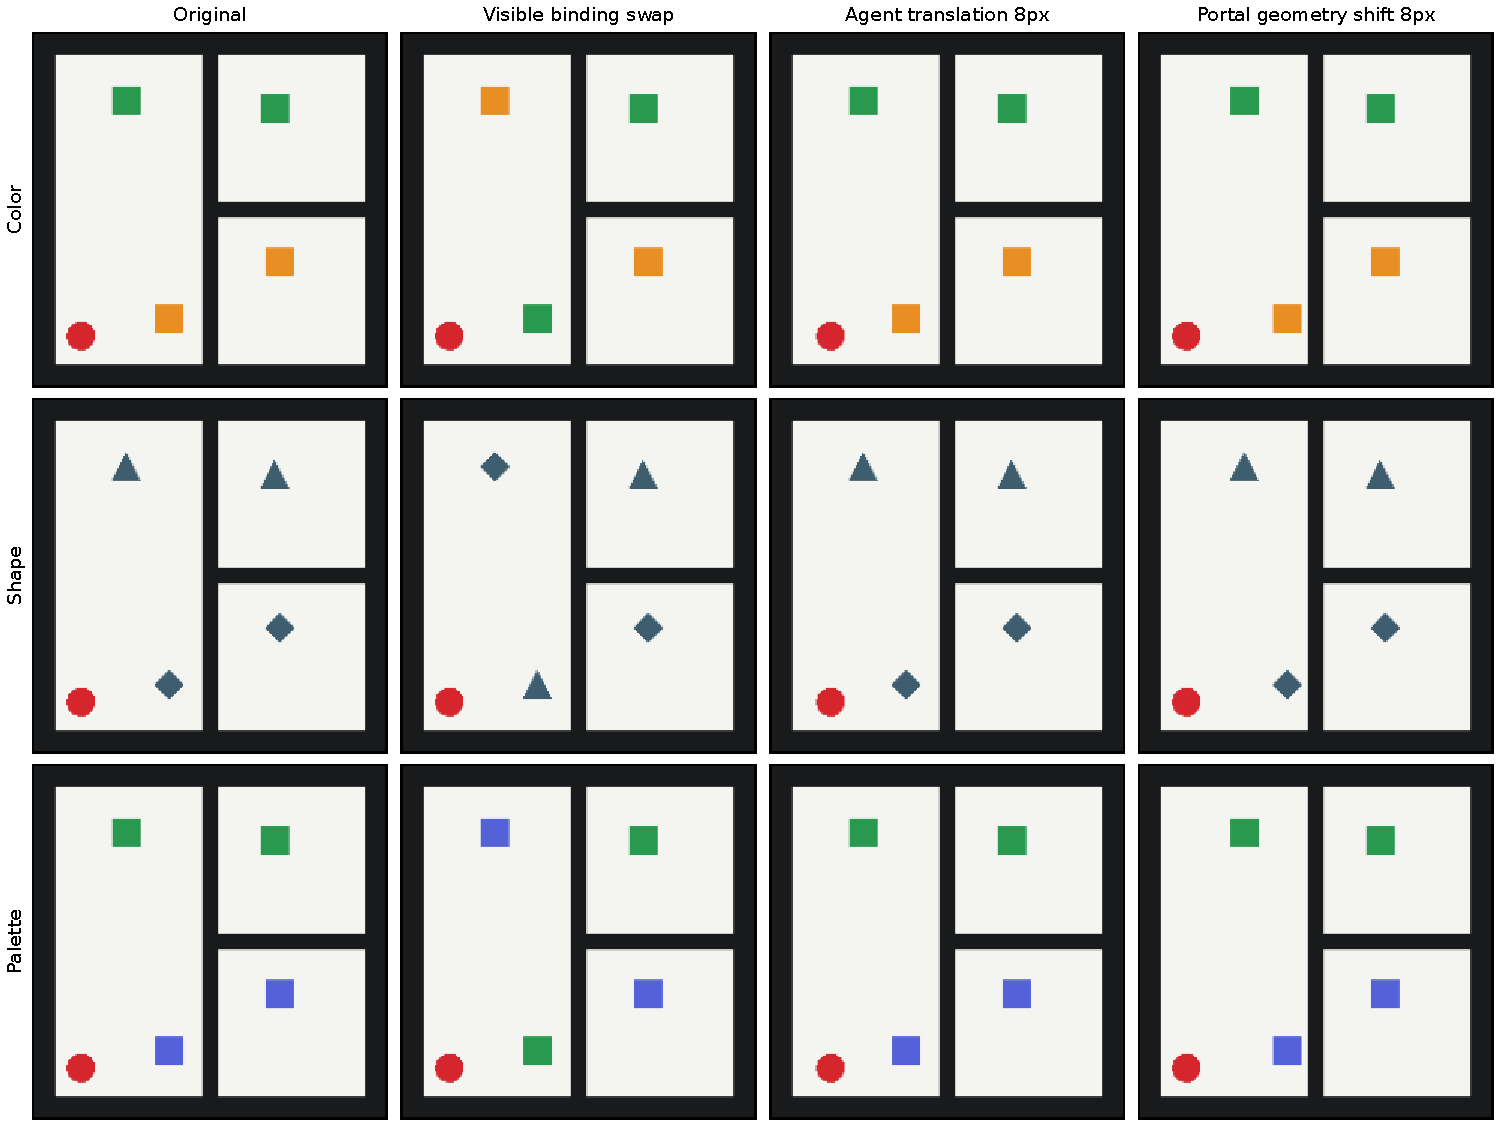
\includegraphics[width=\linewidth]{figures/lewm_portal_swap_states.pdf}
\caption{\textbf{Swapping visible cues changes where the same entrance leads.}
Original worlds, cue swaps, and eight-pixel translations of the agent or
central-room portals, for all three renderings of one illustration geometry.
The swap preserves occupied portal locations and destination-room cues.}
\label{fig:swap-states}
\end{figure}

For the dynamic comparison, each pair receives the same 80 primitive
actions: ten stationary steps, a straight approach to the nearer entrance,
and then zero actions. Both agents remain at identical positions until they
enter that physical portal, at the same step between 15 and 25, then arrive
in different destination rooms. Model forecasts start from observations at
steps 0, 5, and 10, all before the crossing. Subsequent states are predicted
autoregressively using the same normalized five-action blocks in both worlds;
observed post-crossing states are never fed back. We separately encode the
actual trajectories for comparison.

We plot squared distance between the two worlds' projected states and
between their two predicted states. Time zero is the first sampled frame at
or after the true crossing, so the event lies within the preceding five-step
interval. Figure~\ref{fig:swap-curves} shows raw within-model distances and
actual position separation; curves are medians with interquartile bands over
the 16 evaluation geometries.

\begin{figure}[!htbp]
\centering
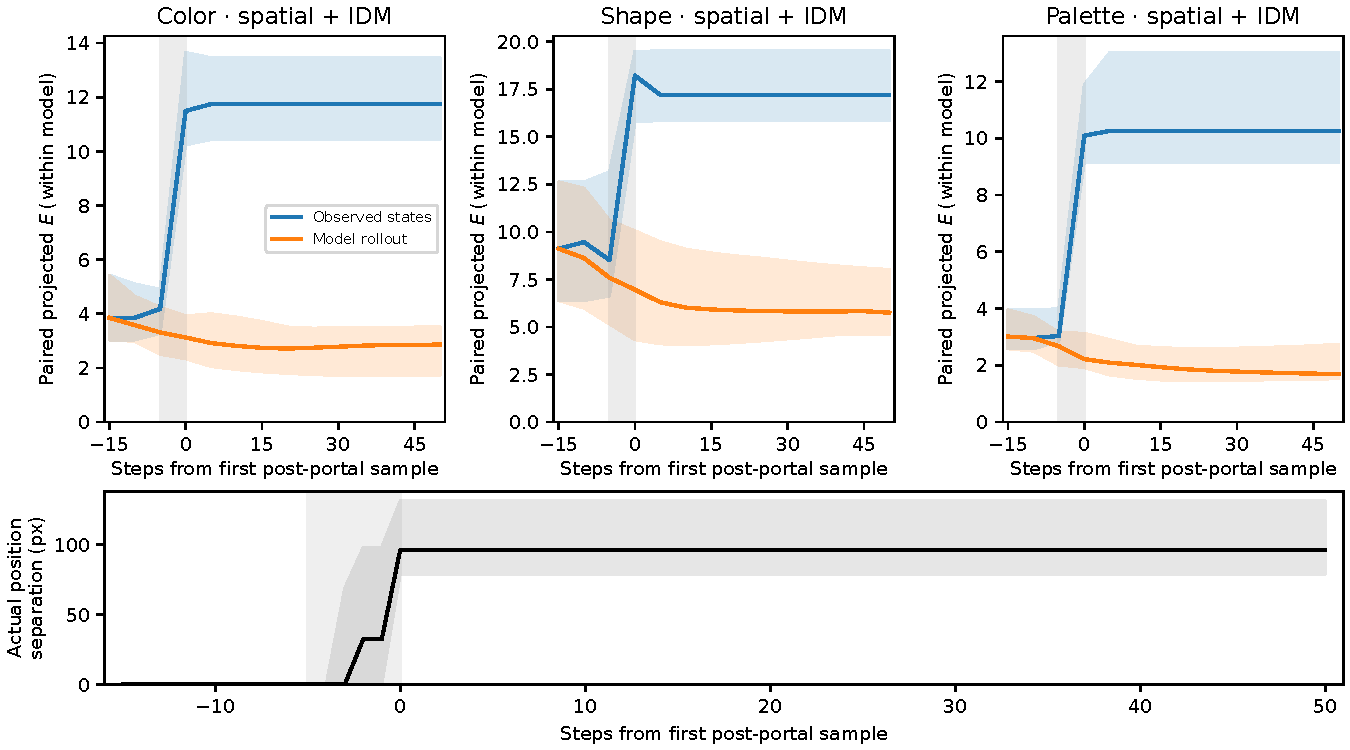
\includegraphics[width=\linewidth]{figures/lewm_portal_swap_raw_event_curves.pdf}
\caption{\textbf{Observed trajectories diverge at the portal; predictions understate the change.}
Top: paired squared latent distances for actual observations (blue) and
open-loop predictions (orange). Bottom: actual position separation, shared
across renderings. Medians and interquartile bands summarize 16 geometries.
The gray interval contains the first portal transition. Latent scales are
interpreted within each model, not across columns.}
\label{fig:swap-curves}
\end{figure}

\begin{table}[!htbp]
\centering
\caption{\textbf{Cue swaps are detectable, but their predicted consequences are attenuated.}
Static ratios use each case's agent-shift energy. The forecast ratio compares
mean predicted and observed separation over the first three post-crossing
samples. Entries show medians [25th, 75th percentiles] across 16 geometries,
not confidence intervals.}
\label{tab:swap}
\renewcommand{\arraystretch}{1.12}
\setlength{\tabcolsep}{4pt}
\begin{tabular*}{\linewidth}{@{\extracolsep{\fill}}lrrr@{}}
\toprule
Variant & Cue swap / agent shift & Portal shift / agent shift & Forecast / observed \\
\midrule
Color & 0.92 [0.71, 1.06] & 5.66 [3.99, 7.34] & 0.25 [0.17, 0.31] \\
Shape & 1.72 [1.16, 2.34] & 5.94 [4.42, 8.04] & 0.42 [0.30, 0.46] \\
Palette & 0.58 [0.39, 0.67] & 3.79 [3.27, 5.69] & 0.18 [0.15, 0.26] \\
\bottomrule
\end{tabular*}
\end{table}

Swaps elicit nonzero responses comparable to an eight-pixel agent shift
(Table~\ref{tab:swap}); the encoder is not cue invariant. Portal translation
produces larger median responses. After crossing, median forecast/observed
separation ratios are .25, .42, and .18 for Color, Shape, and Palette, with
attenuation in every evaluated pair. These rollouts understate the routing
change's consequences, but general prediction error or open-loop contraction
may contribute. A dynamic translation control would help distinguish these
explanations.
